\section{Results}

    This section introduces all the results provided by Alloy through the predicates above. `Check' allows the analysis of the assertions and the verification of them, then `show' displaies the model and verifies its consistency.
    
    \subsection{Data4Help results}
    These predicates for Data4Help verify if a single request returns the data only if the user's answer is positive, and if, in case of multiple request, the data are provided only if the number of people corresponding to some specific filter is greater or equal than 1000 (3 in the model for simplification).\\
  
\begin{lstlisting}[language=alloy]
    check singleRequest for 10
    check multipleRequest for 10 but exactly 8 User
    run show for 10 but exactly 8 User
\end{lstlisting}

    \begin{figure}[H]
        \centering
        \makebox[\textwidth][c]{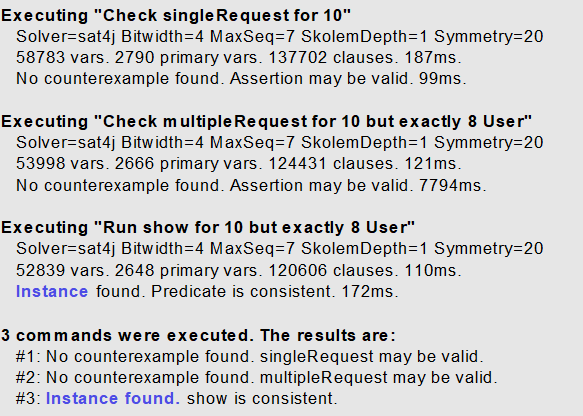
\includegraphics[scale=0.70]{pictures/Results_D4H.png}}
        \caption{ This figure shows the results provided by the analyser after the execution of the predicates above.}
        \label{ fig:D4H-Results }
    \end{figure}
    
    \begin{figure}[H]
        \centering
        \makebox[\textwidth][c]{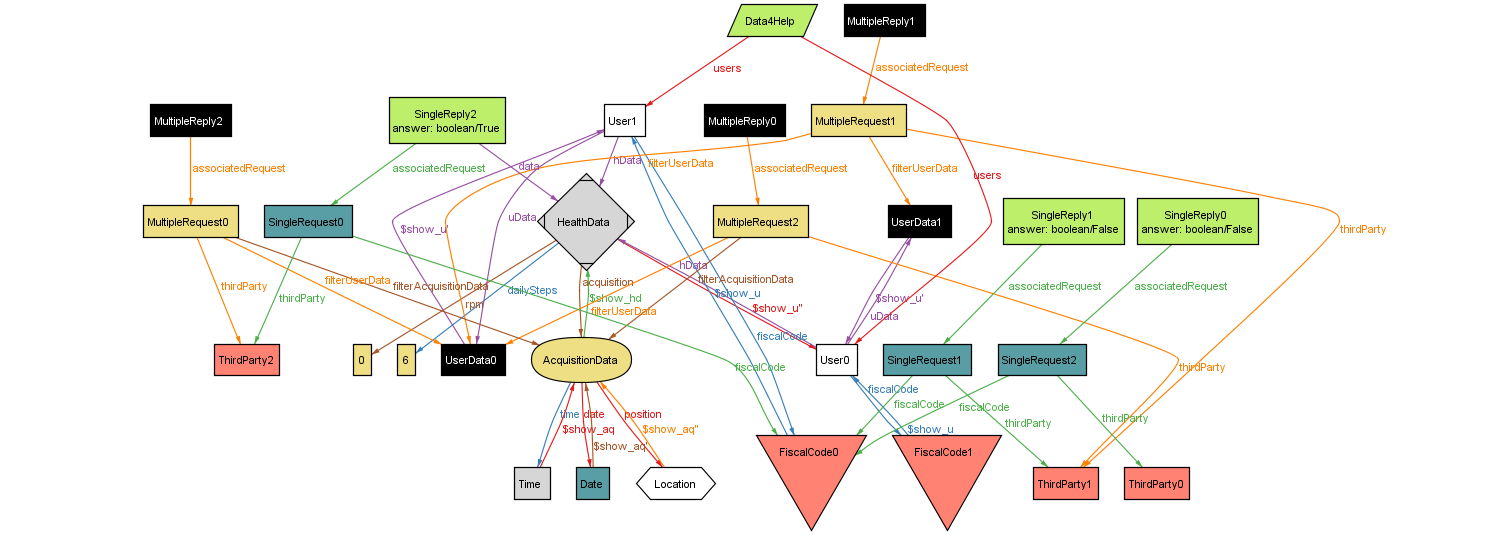
\includegraphics[scale=0.40]{pictures/modelD4H_SingleOk&Not.png}}
        \caption{ This figure represents a model of the world that includes: the case of single request accepted and refused and the case of multiple request refused. }
        \label{ fig:D4H-single-model }
    \end{figure}
    
    \begin{figure}[H]
        \centering
        \makebox[\textwidth][c]{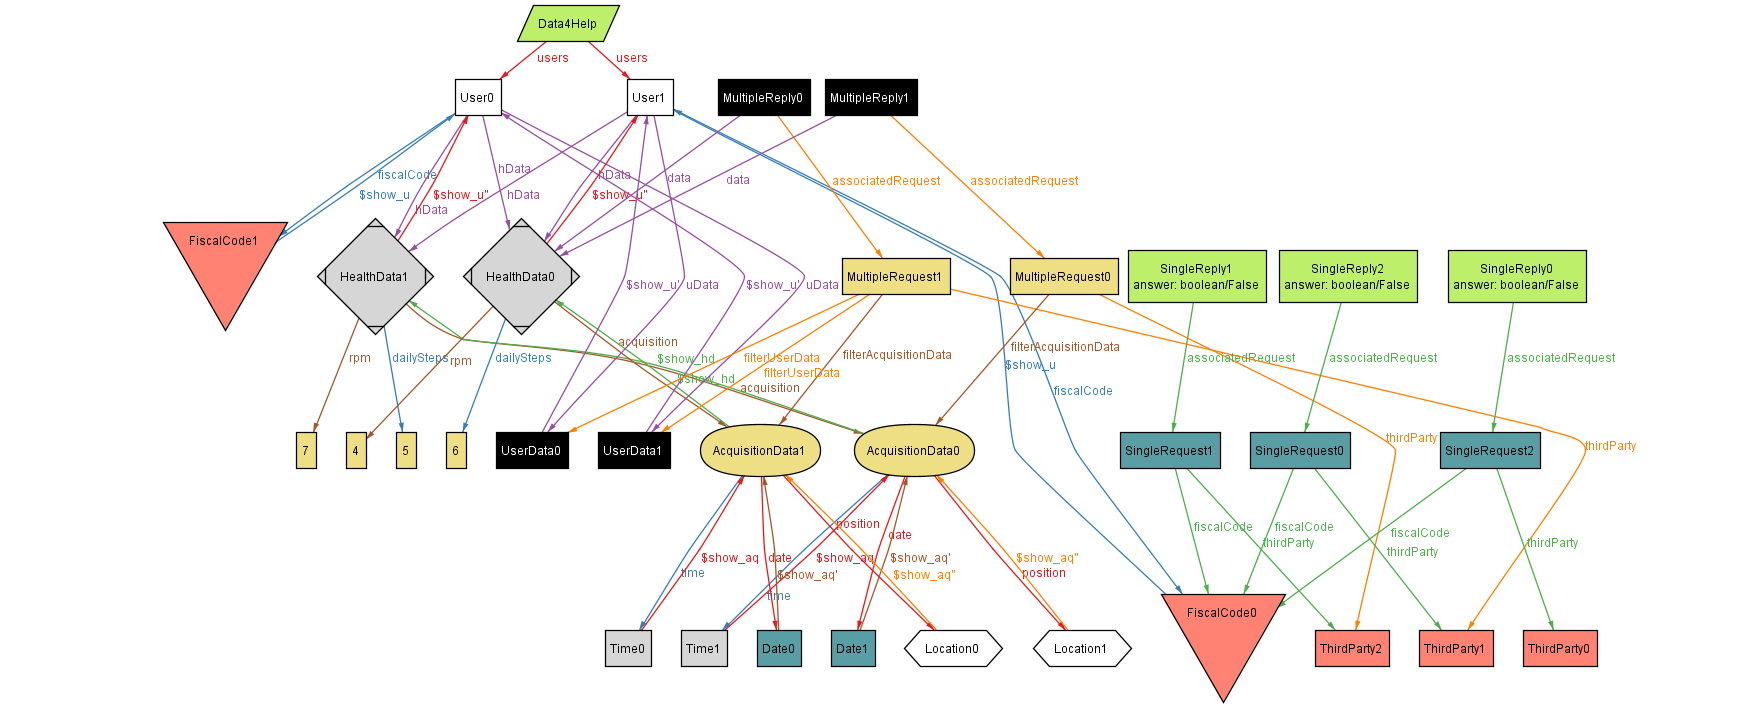
\includegraphics[scale=0.35]{pictures/modelD4H_MulReqOk.png}}
        \caption{ This figure represents a model of the world that includes the case of multiple request accepted.}
        \label{ fig:D4H-multiple-model }
    \end{figure}

    \subsection{AutomatedSOS results}
    On the other hand, the predicates above verify if the model of AutomatedSOS respect the constraint. Therefore, it proves the presence of an ambulance request if and only if a registered user has an hearth frequency too high or too low in relation to some thresholds.\\
    
\begin{lstlisting}[language=alloy]
    check ambulanceRequestWhenBpmNotOutOfBound for 10
    check noAmbulanceWhenBpmOutOfBound for 10
    run show for 10
\end{lstlisting}

    \begin{figure}[H]
        \centering
        \makebox[\textwidth][c]{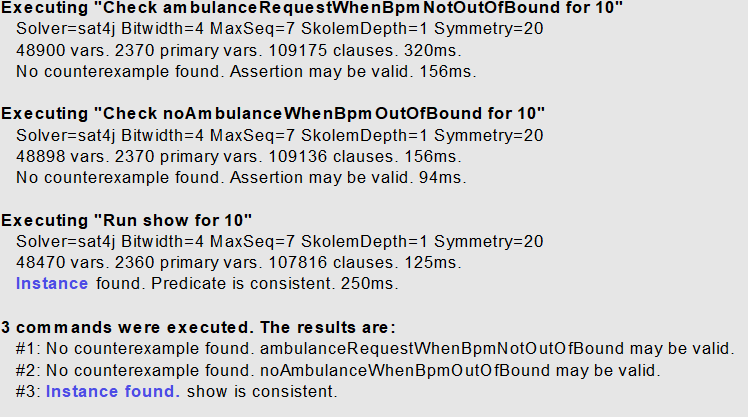
\includegraphics[scale=0.70]{pictures/Results_ASOS.png}}
        \caption{This figure shows the results provided by the analyser after the execution of the predicates above.}
        \label{ fig:ASOS-Results }
    \end{figure}
    
    \begin{figure}[H]
        \centering
        \makebox[\textwidth][c]{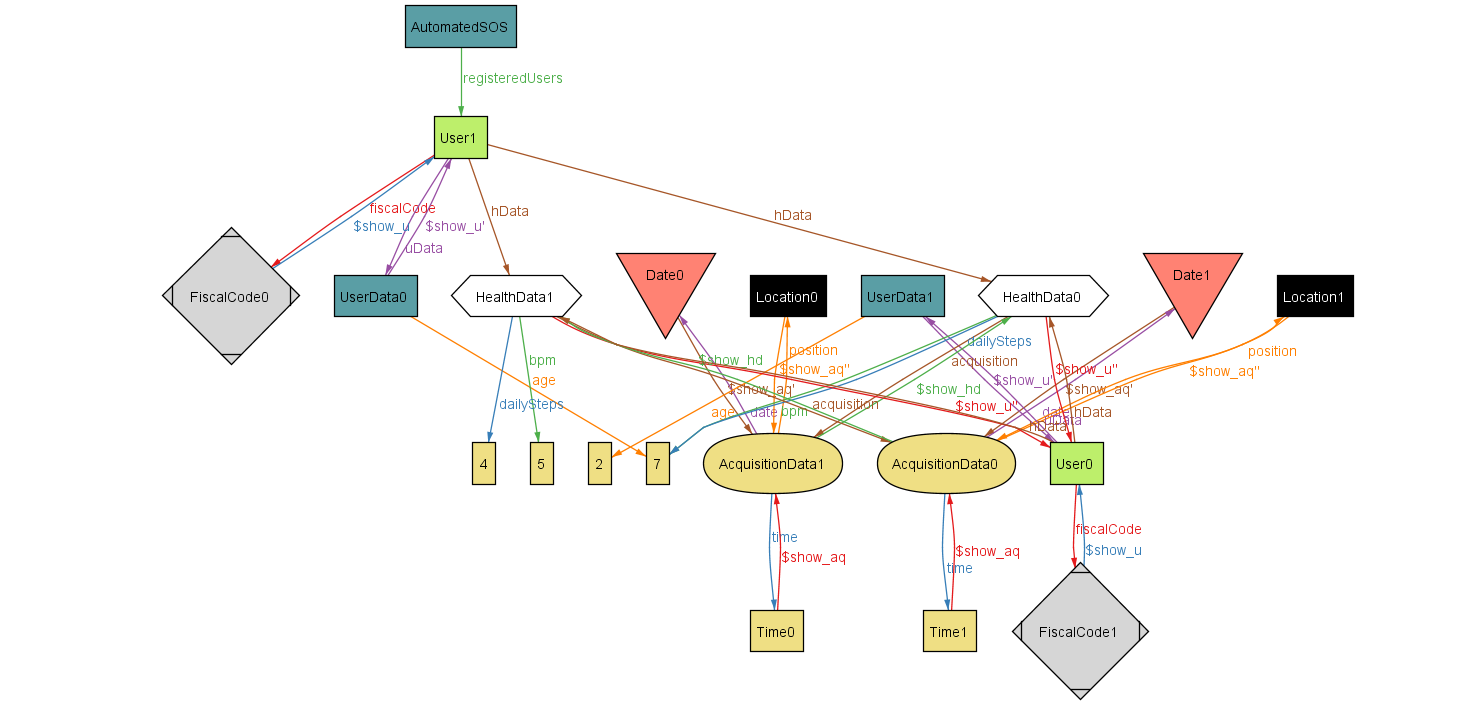
\includegraphics[scale=0.40]{pictures/modelASOS_caseOfBpmOK.png}}
        \caption{This figure shows an instance of the world where an individual has bpm inside the limits, then no ambulance requests have been created. }
        \label{ fig:ASOS-model-bpm-ok }
    \end{figure}
    
    \begin{figure}[H]
        \centering
        \makebox[\textwidth][c]{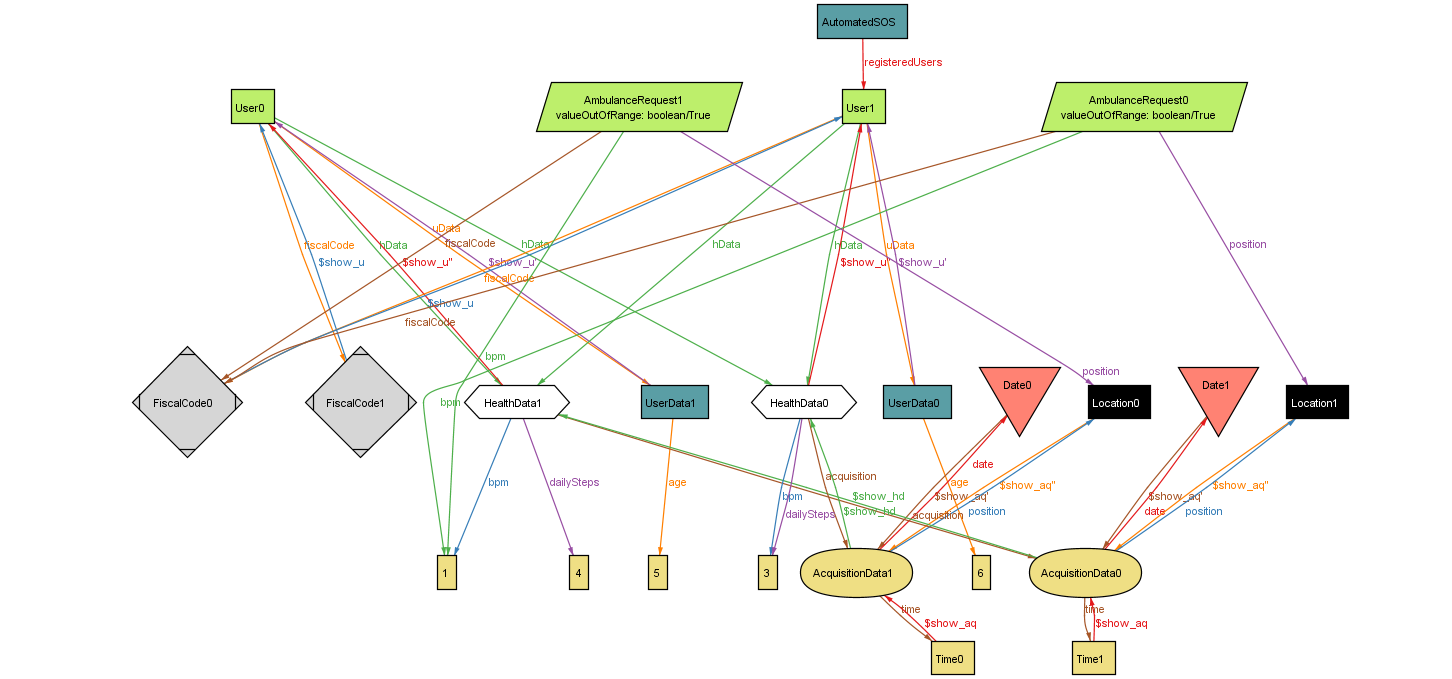
\includegraphics[scale=0.40]{pictures/modelASOS_caseRequest.png}}
        \caption{ In this figure is represented the opposite case of the previous one, it displays the case where one Individual has Bpm out of critical range. }
        \label{ fig:ASOS-model-request }
    \end{figure}

    \subsection{Track4Run results}
    In the last service, Track4Run, the predicate verifies that a visitor can track only the participants enrolled to the race followed by him.
   
\begin{lstlisting}[language=alloy]
    check noVisitorLookingToParticipantsOfDifferentRace for 10
    run show for 10
\end{lstlisting} 
    
    \begin{figure}[H]
        \centering
        \makebox[\textwidth][c]{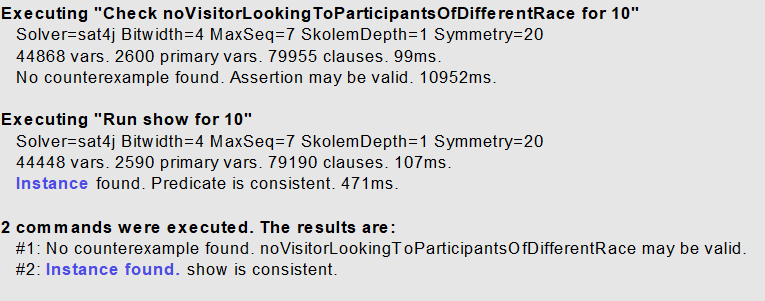
\includegraphics[scale=0.70]{pictures/Results_T4R.png}}
        \caption{This figure shows the results provided by the analyser after the execution of the predicates above. }
        \label{ fig:T4R-Results }
    \end{figure}
    
    \begin{figure}[H]
        \centering
        \makebox[\textwidth][c]{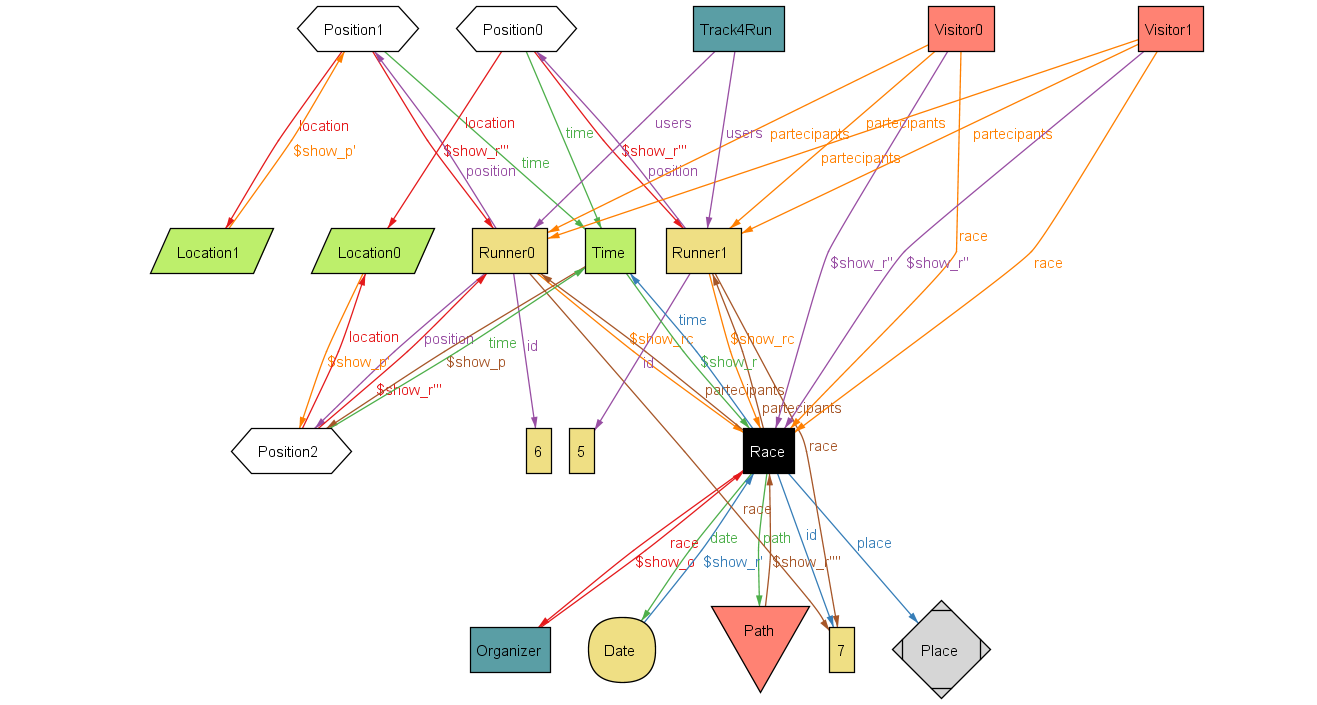
\includegraphics[scale=0.40]{pictures/modelT4R.png}}
        \caption{ This figure represents an instance of the world create by the constraints imposed with the facts. }
        \label{ fig:T4R-model }
    \end{figure}
